\documentclass{ltugboat}
\usepackage[T1]{fontenc}
\usepackage{graphicx}
\usepackage{hologo}
\usepackage{microtype}
\usepackage[hidelinks]{hyperref}

\title{Abstract Diagrams for the Working Mathematician}

\author{Roman Maksimovich}
% \address{Apartment C4, 43 Kam Ping St. \\ Hong Kong, 999077 \\ Hong Kong}
\address{Hong Kong}
\netaddress{r.a.maksimovich (at) gmail.com}

\newcommand{\asy}{\texttt{Asymptote}} 
\newcommand{\smo}{\texttt{smoothmanifold}} 

% Please state if you'd like to receive a physical copy of the TUGboat
% issue or if electronic access suffices.  If you want a physical issue,
% please include the mailing address we should use, as a comment if
% you prefer it not be printed.

% -- Electronic access suffices.

\begin{document}
\maketitle

\begin{abstract}
Within the niche of mathematicians, there's a niche of those who need
to draw diagrams related to pure mathematics.
Within \emph{that} niche there's a niche of people who have experience
in programming and feel comfortable writing code to produce graphics.
This article is for them. It's a survey of the available tools and
a showcase of a library I wrote specifically to simplify the process
of drawing diagrams in differential geometry, topology, set theory, etc.
\end{abstract}

\section{Introduction}

Back in high school, I was attending a seminar on differential geometry,
and I wanted to practice my \LaTeX\ skills by typesetting the lecture
notes. I found myself needing to draw simple surfaces such as those seen
on Figure \ref{fig:manifolds}.

\begin{figure}[ht]
\centering
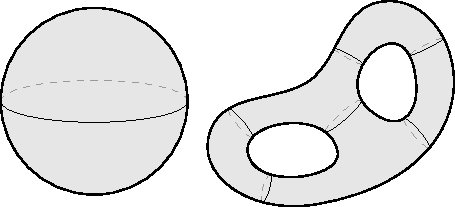
\includegraphics{figures/surfaces.pdf}
\caption{Basic two-dimensional manifolds}
\label{fig:manifolds}
\end{figure}

At that point I realized I wasn't sure how to draw this. I started by
considering some of the available tools:

\begin{itemize}
  \item \textbf{Inkscape} (\url{https://www.inkscape.org})\\
    This is a popular and versatile \acro{GUI} program for drawing vectorized
    graphics, suitable when the diagram is simple enough to be drawn
    by hand with some precision assistance. This assumption holds for
    the left-hand side of Figure~\ref{fig:manifolds}, but not for the
    right-hand side. The reason is that each ``cross section ring'' has
    to be drawn at a precisely calculated position, where it meets its
    bounding paths at equal angles, as illustrated on
    Figure~\ref{fig:close}.\\
    \begin{figure}[ht]
    \centering
    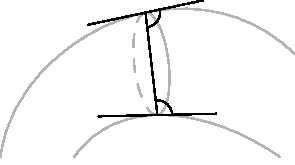
\includegraphics{figures/surface-close.pdf}
    \caption{A good position for drawing a cross section ring, equal angles
      with the tangent lines}
    \label{fig:close}
    \end{figure}
    Besides, it would be useful to tweak the count
    and positions of these ``cross sections'' to see what works best
    for the picture, and this is not something that can be achieved
    with a \acro{GUI} tool like \textbf{Inkscape}. Pass.
  \item \textbf{\LaTeX's \texttt{picture} environment}\\
    There are native drawing capabilities to \LaTeX, but they are
    severely limited. For instance, a straight line segment can be
    drawn like so:\\[5pt]
    \begin{minipage}{0.36\textwidth}
      \begin{verbatim}
\begin{picture}(15,30)
  \put(0,0){\line(1,2){15}}
\end{picture}
      \end{verbatim}
    \end{minipage}
    % \hfill
    \begin{minipage}{0.07\textwidth}
      \begin{picture}(15,20)
        \put(0,0){\line(1,2){15}}
      \end{picture}
    \end{minipage}
    This yields the line shown on the right-hand side. The command
    \verb|\line(m,n){l}| creates a line whose slope is
    $\verb|n|/\verb|m|$ and whose horizontal projection is \verb|l|
    units long.
    However, both \verb|n| and \verb|m| must not exceed 6, and must be
    coprime. The reason for these weird restrictions is the mechanism
    behind the \texttt{picture} environment: instead of producing true
    vector graphics, it tries to assemble the diagram from glyphs
    found in \TeX's fonts, and these fonts only provide a small
    variety of sloped straight lines (if you are reading this article
    digitally, you can zoom in on the straight line above and see that
    it's actually three aligned forward slashes).\\
    To be fair, \texttt{picture} is also capable of drawing an arbitrary
    B\'ezier curve by putting it together from many black squares.
    Still, this is a pretty rudimentary tool unsuited for complicated
    technical drawing, and it's mainly used to define custom
    symbols rather than full diagrams. Pass.
  \item \textbf{The \TikZ\ package} (\url{https://tikz.dev})\\
    For the absolute majority of \TeX\ users, this is the go-to tool
    for technical drawing, and reasonably so. \TikZ\ has a
    comprehensive manual and a rich ecosystem of packages to suit
    virtually your every need. Clearly, both manifolds on
    Figure~\ref{fig:manifolds} can be drawn with \TikZ.\\
    However, my high school self was positively intimidated by the
    \TikZ\ manual (1321 pages?!), and besides, I wanted to write an
    \emph{algorithm} that could calculate the best positions for cross
    section rings, not just a \TeX\ macro. I was fascinated by the
    \textbf{C} programming language at the time, and I wanted to write
    a \emph{function} which would accept two paths as arguments, as
    well as the desired number of cross sections, and return the
    coordinates at which they would look best. \TeX\ certainly tries
    to provide some features of a full programming language, but in
    truth it is more of a markup language, poorly suited for writing
    general-purpose algorithms. Hence, I passed on \TikZ\ also.
    Alternatives to the \TikZ\ package (such as \texttt{pstricks},
    \texttt{xypic}, \texttt{dratex}, etc.) suffer from the same and
    more disadvantages.\\
\end{itemize}

Then, in a stroke of luck, I heard about this vector graphics language
called \asy\ (\url{https://asymptote.sourceforge.io}), and I knew that
it was the one. \asy\ was initially introduced in 2004 at the University of Alberta by
Andy Hammerlindl, John Bowman, and Tom Prince. It is based on the
old \hologo{METAPOST} language, which in turn was based on
Donald Knuth's \hologo{METAFONT} program. However, \asy\ has a \textbf{C}-like
syntax and is indeed a full programming language with data structures,
IEEE floating-point number support, control flow structures like
\texttt{if}, \texttt{for}, and \texttt{while}, etc., as well as very
high-level features such as default arguments and first-class
functions (i.e. functions that can be returned or passed to other
functions as values).

Readers of \TUB\ may have already read about \asy\ in
\cite{fst} and \cite{snd}.

Soon after
learning about \asy, I started writing my own library for this
language, one that I later came to use whenever I needed to create a
diagram in abstract mathematics.

\section{Module \smo}%
\label{sec:smooth}

\subsection{The basics of \asy}%
\label{sub:asy-basics}

An \asy\ user produces graphics by writing code in a file with the
\texttt{.asy} extension, then invoking the \texttt{asy} program on
the command line to compile the code to a picture in a format such as
\acro{PDF}, \acro{SVG}, \acro{PostScript}, or a number of others. Additionally, one may
write \asy\ code directly in a \LaTeX\ document by means of the
\texttt{asymptote} package. This approach removes the necessity to
manually include images, but the code becomes harder to debug.

An example code snippet can look like this:
\begin{center}
\begin{verbatim}
settings.outformat = "eps";
size(4cm);
path p = (0,1) .. (1,0) .. (2,1) .. (3,0);
path q = (0,0) .. (1,1) .. (2,0) .. (3,1);
draw(p ^^ q);
pair[] points = intersectionpoints(p, q);
for (int i = 0; i < points.length; ++i) {
  dot(Label((string)i, align = W),
      points[i], linewidth(4pt));
}
\end{verbatim}
\end{center}

The result of compiling this code is an Encapsulated PostScript file shown in
Figure~\ref{fig:sample}.
\begin{figure}
\centering
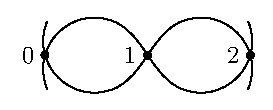
\includegraphics{figures/example.eps}
\caption{A sample picture produced by \asy}
\label{fig:sample}
\end{figure}
Take note of \asy's support of arrays and its native
\texttt{intersectionpoints} function (whereas in \TikZ\ one would load
additional libraries to gain this functionality).

\asy\ has other outstanding features such as powerful
three-dimensional drawing, rich support for mathematical functions,
but most importantly, the ease with which the language can be extended
or modified. In the following subsections, I will outline the most prominent
features of my own library (which
now counts more than 6000 lines of code) and how they allow for
effortless drawing of abstract diagrams.

\subsection{Smooth objects and cross sections}%
\label{sub:cross}

As you recall, my original goal was drawing two-dimensional manifolds
like those in Figure~\ref{fig:manifolds}, so this was the first
functionality I programmed into my library, \smo. A simple torus can
be drawn by writing
\begin{verbatim}
import smoothmanifold;
smooth s = smooth(
  ellipse((0,0), 2, 1)
).addhole(
  ellipse((0,0), 1.1, .37),
  sections = new real[][]{
    r(0, 60, 3), r(90, 90, 1),
    r(180, 60, 3), r(270, 90, 1)
  }
);
config.section.freedom = .9;
size(5cm);
draw(s, dpar(
  mode = free, viewdir = 2.3*dir(90)
));
\end{verbatim}

Compiling this code (assuming that the file
\texttt{smoothmanifold.asy} is located where \asy\ can find it) yields
the picture in Figure~\ref{fig:torus}.

\begin{figure}[h]
\centering
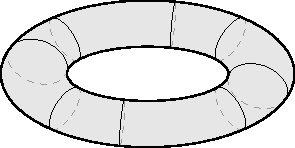
\includegraphics{figures/torus.pdf}
\caption{A torus}
\label{fig:torus}
\end{figure}

You can see that the code is relatively high-level: instead of drawing
cross section rings manually, we build a \emph{smooth object} with the
\texttt{smooth} constructor, then add a hole to it with
\texttt{addhole}, whose \texttt{sections} parameter allows to
configure the positions of cross sections. It's not crucial to
understand what exactly goes on in that \texttt{real[][]} array,
suffice it to say that it tells \smo\ roughly where we want it to draw
cross section rings around the given hole.

After creating the smooth object and assigning it to the \texttt{s}
variable, we set some configuration values. The
\texttt{config.section.freedom} value determines how much leeway is
given to the section finding algorithm (to be explained later), and the \texttt{size()}
function allows us to set the picture's size.

Finally, we \texttt{draw} the smooth object, providing a \texttt{dpar}
(\textbf{d}rawing \textbf{par}ameters) structure, where we specify how
the object (and its cross sections) should be drawn. The
\texttt{viewdir} parameter is the ``direction of view'', and it helps
coordinate the widths of different cross section rings, such that
together they create the illusion of a 3D object.

Interested readers may consult the full\linebreak \smo\ manual
\cite{manual} for more detail.

\subsection{The cross section finding algorithm}%
\label{sub:find}

Although I don't wish to delve too deep into technical aspects, I think
the cross section finding algorithm merits a short discussion. The relevant
\smo\ function is
\begin{verbatim}
pair[][] sectionparams
(path g, path h, int n, real r, int p)
\end{verbatim}
It tries to find the best positions for \texttt{n} cross sections
between the paths \texttt{g} and \texttt{h}, and it does so by first
splitting both paths into regions, as seen in Figure~\ref{fig:regions}

\begin{figure}[h]
\centering
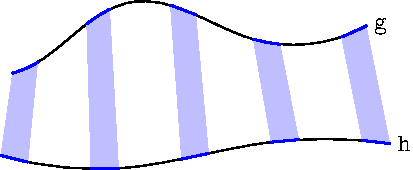
\includegraphics{figures/regions.pdf}
\caption{\texttt{n} regions (blue) are formed between the paths
  \texttt{g} and \texttt{h}}
\label{fig:regions}
\end{figure}

Here \texttt{n} is set to 5, so five regions are selected in the
space between
the paths, and the algorithm will try to find an optimal
position for a cross section in each region.
The \texttt{real r} parameter of the
\texttt{sectionparams} function determines the relative\linebreak width
of these regions. If \texttt{r = 0}, each region is a line, and
there is no choice. If \texttt{r = 1}, then the regions cover
all space between \texttt{g} and \texttt{h}. In a sense,
\texttt{r} is the ``freedom of choice'', hence its default value is
the \texttt{config.section.freedom} settings option.

Then, the algorithm proceeds to select \texttt{p} sample points along either edge of
each region, and search for the optimal section position by minimizing
a loss function. This is illustrated in Figure~\ref{fig:search}.

\begin{figure}[h]
\centering
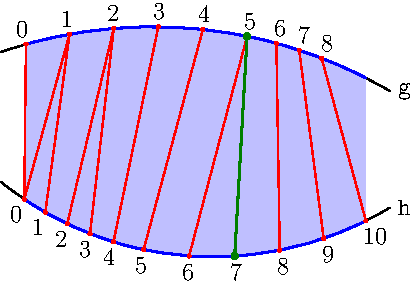
\includegraphics{figures/search.pdf}
\caption{Selecting the optimal section position within one region}
\label{fig:search}
\end{figure}

As you can see, not every combination of points is checked. This is a
heuristic optimization based on the fact that ``good'' cross sections
usually connect points whose indices are close. This allows the
algorithm to run in $O(n p)$ time, whereas the naive implementation is
$O(n p^2)$.

\bibliographystyle{tugboat}
\bibliography{main}

\makesignature
\end{document}
